\documentclass[12pt]{article}

%***************************************************************************************************
% Math
\usepackage{fancyhdr} 
\usepackage{amsfonts}
\usepackage{amsmath}
\usepackage{amssymb}
\usepackage{amsthm}
%\usepackage{dsfont}

%***************************************************************************************************
% Macros
\usepackage{calc}

%***************************************************************************************************
% Commands and Custom Variables	
\newcommand{\problem}[1]{\hspace{-4 ex} \large \textbf{Problem #1} }
\let\oldemptyset\emptyset
\let\emptyset\varnothing
\newcommand{\norm}[1]{\left\lVert#1\right\rVert}
\newcommand{\sint}{\text{s}\kern-5pt\int}
\newcommand{\powerset}{\mathcal{P}}
\renewenvironment{proof}{\hspace{-4 ex} \emph{Proof}:}{\qed}
\newcommand{\RR}{\mathbb{R}}
\newcommand{\NN}{\mathbb{N}}
\newcommand{\QQ}{\mathbb{Q}}
\newcommand{\ZZ}{\mathbb{Z}}
\newcommand{\CC}{\mathbb{C}}


%***************************************************************************************************
%page
\usepackage[margin=1in]{geometry}
\usepackage{setspace}
%\doublespacing
\allowdisplaybreaks
\pagestyle{fancy}
\fancyhf{}
\rhead{Shaw \space \thepage}
\setlength\parindent{0pt}

%***************************************************************************************************
%Code
\usepackage{listings}
\usepackage{courier}
\lstset{
	language=Python,
	showstringspaces=false,
	formfeed=newpage,
	tabsize=4,
	commentstyle=\itshape,
	basicstyle=\ttfamily,
}

%***************************************************************************************************
%Images
\usepackage{graphicx}
\graphicspath{ {images/} }
\usepackage{float}

%tikz
\usepackage[utf8]{inputenc}
\usepackage{pgfplots}
\usepgfplotslibrary{groupplots}

%***************************************************************************************************
%Hyperlinks
%\usepackage{hyperref}
%\hypersetup{
%	colorlinks=true,
%	linkcolor=blue,
%	filecolor=magenta,      
%	urlcolor=cyan,
%}

\begin{document}
	\thispagestyle{empty}
	
	\begin{flushright}
		Sage Shaw \\
		m565 - Fall 2017 \\
		\today
	\end{flushright}
	
{\large \textbf{HW 5}}\bigbreak

\problem{1 (Natural cubic spline) (a)} 

	From our natural end condition we know that $s_1^{\prime\prime}(x_2)=0$. Thus \\$-\tfrac{3}{2} + 6d_1(4-3) = 0$ gives us that $d_1 = \tfrac{1}{4}$. Since $s_1$ interpolates the point $(4,0)$ we know that $s_1(4)=0$ so 

	\begin{align*}
		0 & = 1 + b_1(4-3) - \tfrac{3}{4}(4-3)^2 + \tfrac{1}{4}(4-3)^3\\
		& = \tfrac{1}{2} + b_1 \\
		-\tfrac{1}{2} & = b_1
	\end{align*}

	Frome the condition that $s_0^{\prime\prime}(3) = s_1^{\prime\prime}(3)$ we have that
	\begin{align*}
		s_0^{\prime\prime}(3) & = s_1^{\prime\prime}(3) \\
		6d_0(3-1) & = -\tfrac{3}{2} + 6d_1(3-3) \\
		d_0 & = -\tfrac{1}{8}
	\end{align*}

	From the condition that $s_0^\prime(3) = s_1^\prime(3)$ we have
	\begin{align*}
		s_0^\prime(3) & = s_1^\prime(3)\\
		b_0 - \tfrac{3}{8}(3-1)^2 & = b_1 = -\tfrac{1}{2} \\
		b_0 & = 1
	\end{align*}
	
	Thus our values are $b_0 = 1, d_0 =-\tfrac{1}{8}, b_1 = -\tfrac{1}{2}$, and $ d_1 = \tfrac{1}{4}$. 
	
\problem{1 (b)} Using the Newton's divided difference table we have

	\begin{center}
		\begin{tabular}{|c|c|c|c|}\hline
			$x_i$ & $f[\cdot]$ & $f[\cdot,\cdot]$ & $f[\cdot,\cdot,\cdot]$ \\ \hline
			1 & 0 & & \\ \hline
			3 & 1 & $\tfrac{1}{2}$ &\\ \hline
			4 & 0 & -1 & $0-\tfrac{1}{2}$ \\ \hline
		\end{tabular}
	\end{center}
	so our global interpolating polynomial is 
	$$
	p_2 = 0 + \tfrac{1}{2}(x-1) - \tfrac{1}{2}(x-1)(x-3) = \tfrac{1}{2}(-4+5x-x^2)
	$$
	Then
	\begin{align*}
		\int_1^4 [s^{\prime\prime}(x)]^2 dx & = \int_1^3 [s_0^{\prime\prime}(x)]^2 dx + \int_3^4 [s_1^{\prime\prime}(x)]^2 dx \\
		& = \int_1^3 [-\tfrac{6}{8}(x-1)]^2 dx + \int_3^4 [-\tfrac{3}{2} + \tfrac{3}{2}(x-3)]^2 dx \\
		& = \int_1^3 \tfrac{9}{16}(x-1)^2 dx + \int_3^4 [\tfrac{3}{2}(x-4)]^2 dx \\
		& = \int_1^3 \tfrac{9}{16}(x-1)^2 dx + \int_3^4 \tfrac{9}{4}(x-4)^2 dx \\
		& = \tfrac{3}{16}(x-1)^3 \Big\vert_1^3 + \tfrac{3}{4}(x-4)^3 \Big\vert_3^4 \\
		& = \tfrac{3}{2} + \tfrac{3}{4} \\
		& = \tfrac{9}{4}
	\end{align*}
	and 
	\begin{align*}
		\int_1^4 [p_2^{\prime\prime}(x)]^2 dx & = \int_1^4 [\tfrac{1}{2}(-2)]^2 dx \\
		& = \int_1^4 1 dx \\
		& = 3
	\end{align*}
	Indeed $\int_1^4 [s^{\prime\prime}(x)]^2 dx < \int_1^4 [p_2^{\prime\prime}(x)]^2 dx$.
	
\problem{2 (Periodic Cubic Spline) (a)}
	
	As in the general case for $k = 1, ..., n-1$ we have
	$$
	h_kd_{k-1} + 2(h_{k+1} + h_{k})d_k + h_{k-1}d_{k+1} = 3(h_k\delta_{k-1} + h_{k-1}\delta_{k})
	$$
	In order to solve the system we need two more equations which we will get from our periodic end conditions. From the condition $s_0^\prime(x_0) = s_{n-1}^\prime(x_n)$ we know that $d_0 = d_n$. From $s_0^{\prime\prime}(x_0) = s_{n-1}^{\prime\prime}(x_n)$ we know that
	\begin{align*}
		2c_0 & = 2c_{n-1} + 6b_{n-1}h_{n-1} \\
		c_0h_0h_{n-1} & = c_{n-1}h_0h_{n-1} + 3b_{n-1}h_{n-1}h_0h_{n-1} \\
		(3\delta_0 - 2d_0 - d_1)h_{n-1} & = (3\delta_{n-1} - 2d_{n-1} - d_n)h_{0} + 3(d_{n-1} -2\delta_{n-1} + d_n)h_{0} \\
		3(h_{n-1}\delta_0 + h_0\delta_{n-1}) & = 2h_{n-1} d_0 + h_{n-1}d_1 + h_0d_{n-1} + 2h_0d_n 
	\end{align*}
	
\problem{2 (b)}

	From part (a) we have the linear system $A\vec{d} = \vec{b}$
	$$
	\begin{bmatrix}
	1 & & & \dots & -1\\
	h_1 & 2(h_1+h_0) & h_0\\
	& \ddots & \ddots & \ddots \\
	& & h_{n-1} & 2(h_{n-1}+h_{n-2}) & h_{n-2} \\
	2h_{n-1} & h_{n-1} & & h_0 & 2h_0 \\
	\end{bmatrix}
	\begin{bmatrix}
	d_0 \\
	d_1 \\
	\vdots \\
	d_{n-1} \\
	d_n \\
	\end{bmatrix}
	=
	\begin{bmatrix}
	0 \\
	3(h_1\delta_{0} + h_{0}\delta_{1}) \\
	\vdots \\
	3(h_{n-1}\delta_{n-2} + h_{n-2}\delta_{n-1}) \\
	3(h_{n-1}\delta_0 + h_0\delta_{n-1}) \\
	\end{bmatrix}	
	$$
	
\problem{2 (c)} Code for periodic piecewise cubic spline:
	\begin{lstlisting}
def piecewise_interp(xs, ys, us):
	#periodic piecewise interpolation
	
	#sort the data
	xs = np.array(xs)
	p = xs.argsort()
	xs = xs[p]
	ys = np.array(ys)[p]
	us = np.sort(us)
	
	n = len(xs)
	hs = xs[1:] - xs[:-1]
	
	delta = (ys[1:] - ys[:-1]) / hs
	
	A = np.zeros( (n,n) )
	for i in range(1, n-1):
		A[i, i-1] = hs[i]
		A[i, i] = 2*(hs[i]+hs[i-1])
		A[i, i+1] = hs[i-1]
	A[n-1, 0] = 2*hs[n-2]
	A[n-1, 1] = hs[n-2]
	A[n-1, n-2] = hs[0]
	A[n-1, n-1] = 2*hs[0]
	
	B = np.zeros( (n, 1) )
	for i in range(1, n-1):
		B[i] = 3*( hs[i]*delta[i-1] + hs[i-1]*delta[i] )
	
	A[0,0] = 1
	A[0,n-1] = -1
	B[n-1] = 3*( hs[-1]*delta[0] + hs[0]*delta[-1] )
	
	d = np.linalg.solve(A, B)
	d.shape = (n,)
	
	b = (d[:-1] -2*delta + d[1:])/(hs*hs)
	c = (3*delta - 2*d[:-1] - d[1:])/(hs)
	
	f = np.zeros( len(us) )
	j = 0
	for i, u in enumerate(us):
		while xs[j+1] < u:
			j += 1
			if j >= n-1:
				j = n-2
				break
		dis = u - xs[j] 
		f[i] = ys[j] + d[j]*dis + c[j]*dis**2 + b[j]*dis**3
	return f
	\end{lstlisting}
	
\problem{2 (d)} In figure (\ref{hw5_p2_fig1}) can be seen sample points of $f(x) = \sin(\pi(x-0.01))$ in blue, the periodic cubic spline in red, and the not-a-knot cubic spline in green. The periodic cubic spline appears to be roughly as good an approximation of $f$ as the not-a-knot cubic spline.

	\begin{figure}[H]
		\caption{Plot of sample points from $f(x)$, the periodic cubic spline, and the not-a-knot cubic spline}
		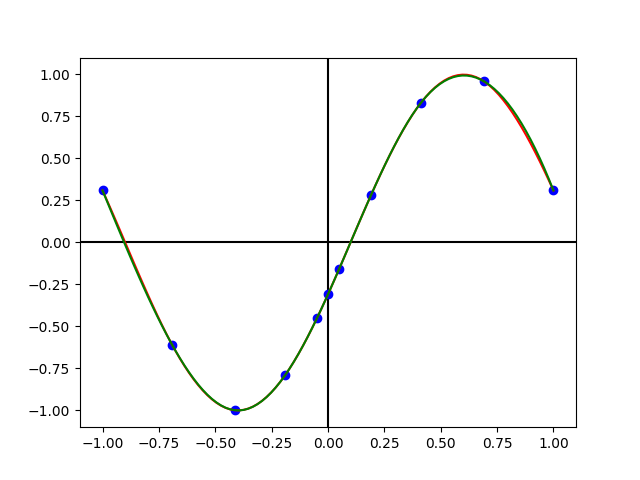
\includegraphics[width=0.80\textwidth]{hw5_p2_fig1}
		\label{hw5_p2_fig1}
		\centering
	\end{figure}


	The code that was used to generate figure (\ref{hw5_p2_fig1}) appears below
	\begin{lstlisting}
def p2d():
	xs = []
	for i in range(0,6):
		xs.append( np.sin(np.pi * i / 10) - 1 )
	for i in range(6, 11):
		xs.append( 1 - np.sin(np.pi * i / 10) )
	xs = np.array(xs)
	ys = np.sin( np.pi*(xs - 0.1) )
	us = np.linspace(-1, 1, 100)
	fs = piecewise_interp(xs, ys, us)
	
	plt.plot( (-100, 100), (0,0), 'k-')
	plt.plot( (0,0), (-100, 100), 'k-')
	plt.plot( xs, ys, 'bo')
	plt.plot( us, fs, 'r-')
	
	cs = CubicSpline(xs,ys)
	plt.plot(us, cs(us), 'g-')
	
	plt.xlim( (-1.1, 1.1) )
	plt.ylim( (-1.1, 1.1) )
	plt.show()
	\end{lstlisting}
	
\problem{3} In figure (\ref{hw5_p3_fig1}) the sample points can be seen in blue, the piecewise-linear interpolation can be seen in green and the periodic cubic spline interpolation can be seen in red.
	
	\begin{figure}[H]
		\caption{Plot of sample points from, the parametric periodic piecewise-cubic spline, and the peicewise-linear interpolation.}
		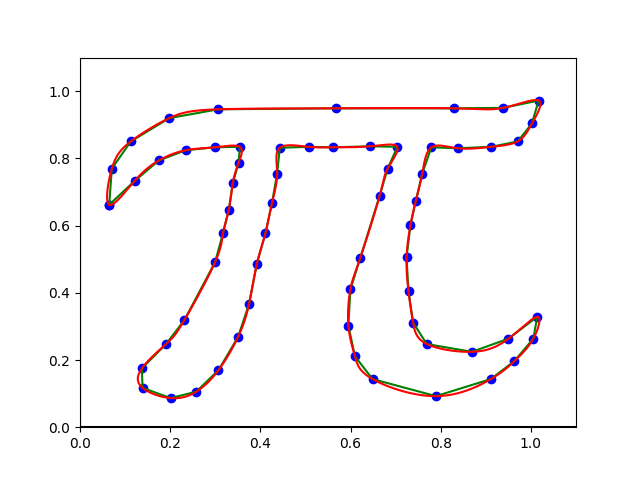
\includegraphics[width=0.80\textwidth]{hw5_p3_fig1}
		\label{hw5_p3_fig1}
		\centering
	\end{figure}
	
	The code that generated figure (\ref{hw5_p3_fig1}) appears below.
	
	\begin{lstlisting}
def p3():
	str = open('res/hw5_DotToDot.txt', 'r').read()
	x = []
	y = []
	for l in str.split('\n'):
		xy = l.split('\t')
		x.append( float(xy[0]))
		y.append( float(xy[1]))
	t = np.linspace(0, 1, len(x))
	u = np.linspace(0, 1, len(x)*100)
	fx = piecewise_interp(t, x, u)
	fy = piecewise_interp(t, y, u)
	
	plt.plot( (-100, 100), (0,0), 'k-')
	plt.plot( (0,0), (-100, 100), 'k-')
	plt.plot( x, y, 'bo')
	plt.plot( x, y, 'g-')
	plt.plot( fx, fy, 'r-')
	
	plt.xlim( (0, 1.1) )
	plt.ylim( (0, 1.1) )
	plt.show()
	\end{lstlisting}
	
	
\problem{4} Figure (\ref{hw5_p4_fig1}) shows topographical data of a two-ravine drainage from Upper State NY (purple), along with the interpolating radial basis function thin plate spline (surface from yellow to red).

	Figure (\ref{hw5_p4_fig2}) shows the same data (red points) in a contour plot of the approximated depth of the surface.

	\begin{figure}[h]
		\caption{Topographical data of two-ravine drainage from Upper State NY, along with the interpolating radial basis function thin plate spline.}
		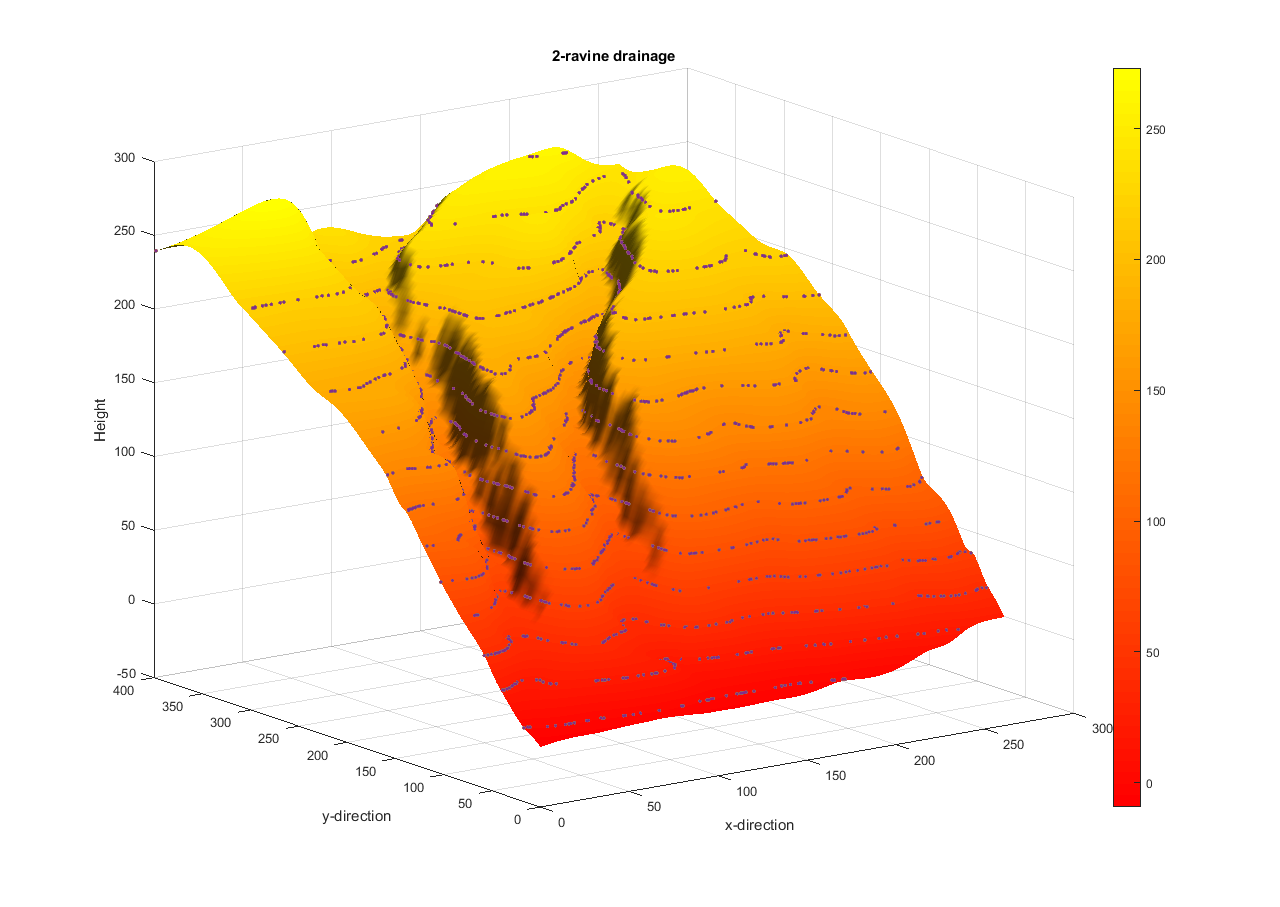
\includegraphics[width=1.0\textwidth]{hw5_p4_fig1}
		\label{hw5_p4_fig1}
		\centering
	\end{figure}

	\begin{figure}[h]
		\caption{Topographical data of two-ravine drainage from Upper State NY, along with the interpolating radial basis function thin plate spline.}
		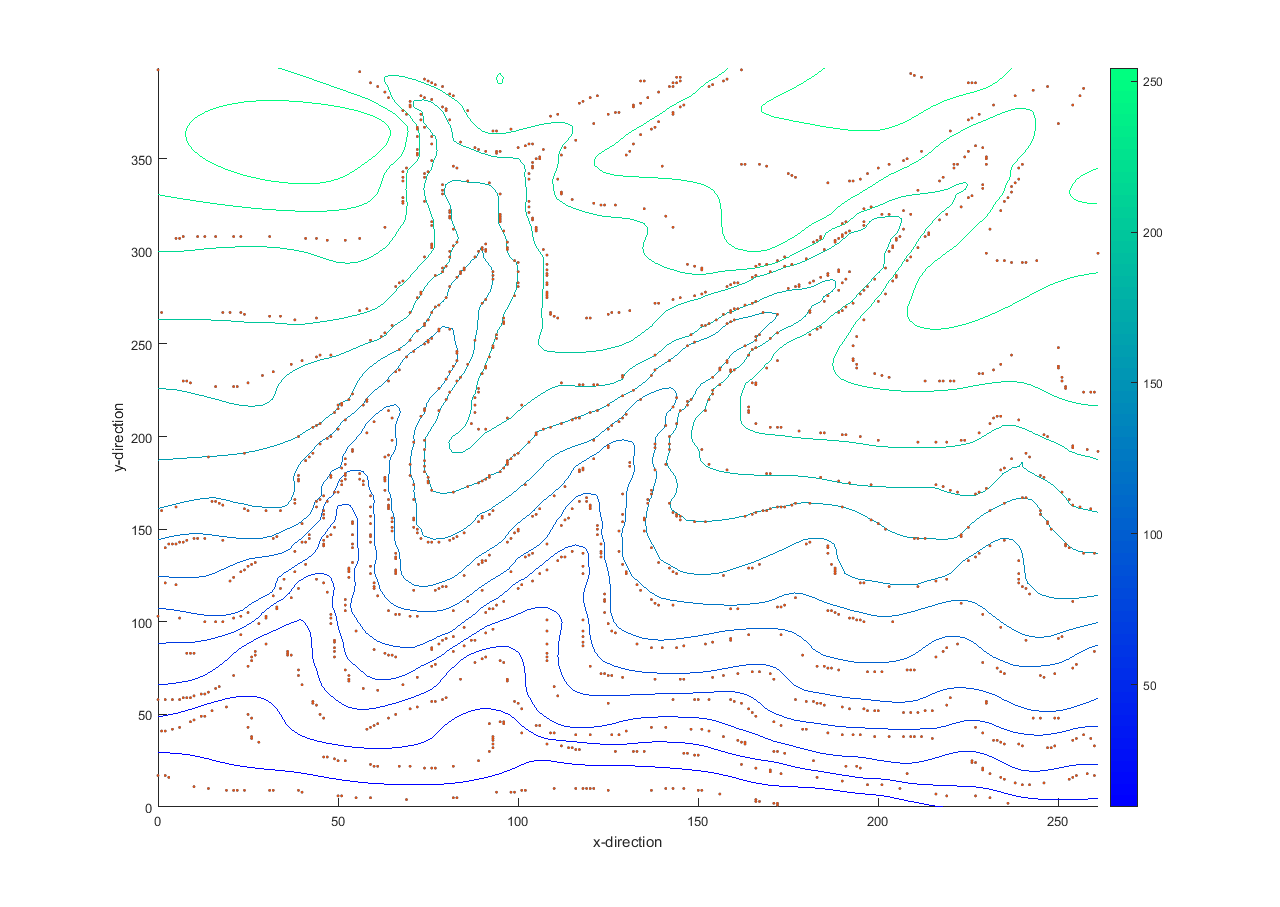
\includegraphics[width=1.0\textwidth]{hw5_p4_fig2}
		\label{hw5_p4_fig2}
		\centering
	\end{figure}

\problem{5 (Piecewise quadratic interpolation)} Each paraboloa in a piecewise quadratic is uniquely determined by three pieces of information. We would like each parabola to interpolate the points (2 peices of information) while being as smooth as possible. We can only require that the first derivatives be equal. To require the second derivatives to be equal would create an over determined system. Let each peice of our piecewise quadratic function be defined 

$$
s_j(x) = y_j + d_j(x-x_j) + c_j(x-x_j)^2 \text{ when } x_j \leq x \leq x_{j+1}
$$

where $(x_j,y_j)$ are the points to be interpolated and $d_j$ is the derivative of $s_j$ and $s_{j+1}$ at $x_j$. Define $h_j = (x_{j+1}-x_j)$ and $\delta_j = (y_{j+1}-y_j)/h_j$, then
\begin{align*}
	s_j(x_{j+1}) & = s_{j+1}(x_{j+1}) \\
	y_j + d_jh_j + c_jh_j^2 & = y_{j+1} \\
	d_j + c_jh_j = \delta_j \\
	c_j & = \frac{\delta_j - d_j}{h_j}
\end{align*} 
and 
\begin{align*}
	s_j^\prime(x_{j+1}) & = s_{j+1}^\prime(x_{j+1}) \\
	d_j + 2c_jh_j & = d_{j+1} \\
	c_j & = \frac{d_{j+1} - d_j}{2h_j}
\end{align*}
Using both of these equations we obtain
\begin{align*}
	\frac{d_{j+1} - d_j}{2h_j} & = \frac{\delta_j - d_j}{h_j} \\
	h_j(d_{j+1} - d_j) & = 2h_j(\delta_j - d_j) \\
	d_j + d_{j+1} & = 2\delta_j
\end{align*}
These conditions hold for $j=0, ..., n-1$. Thus we have $n$ equations and $n-1$ unknowns. One more condition will completely determine the system. We could for example require $s_0(x_0) = s_{n-1}(x_n)$ but then it may not be smooth. We coulde choose the derivative at one of the points, but then we have no control over the derivatives at the end points. If we set the derivative at one of the points (say it is zero for example, an analogue to the natrual cubic case) we have no control over the derivative at the other end point. \bigbreak

In the cubic case, we have more control and flexibility over the behavior of our spline at the end points. The big O order is the same since the bulk of the work is done in solving the $(x+1)\times(n+1)$ linear system.

\problem{6 (Barycentric trigonometric interpolation) (a)}

	Below is my code for the barycentric trigonometric interpolation.
	
	\begin{lstlisting}
def trig_interp(y, u):
	N = len(y)
	if N%2 == 0:
		raise ValueError("y must contain an odd number of values.")
	k = np.linspace(0, 2*np.pi, N, endpoint=False)
	f = []
	sign = np.array( [ (-1)**k for k in range(0,N)] )
	for t in u:
		if t in k:
			p = y[ int(np.argwhere(k==t)) ]
		else:
			denominator = sign / np.sin( (t - k)/2 )
			numerator = denominator * y
			p = np.sum(numerator)/np.sum(denominator)
		f.append(p)
	return f
	\end{lstlisting}
	
\problem{6 (b)} The code above is verified by interpolating the function $f(t)=\sin(2t)\cos(3t)$ by sampling it at 11 equally spaced points. Plots of the interpolating function and the origional function appear in figure (\ref{hw5_p6_fig1}). The function $f$ is in green and the trigonometric interpolation was graphed in red but is such a close approximation that it is not visible. The points in blue are the sample points. \bigbreak

In figure (\ref{hw5_p6_fig2}) can be seen the error $f-p$ where $p$ is the trigonometric interpolation. As expected, the maximum error is less than $2 \times 10^{-15}$, a very good approximation indeed.

\begin{figure}[h]
	\caption{$f(t)=\sin(2t)\cos(3t)$ and the trigonometric interpolation}
	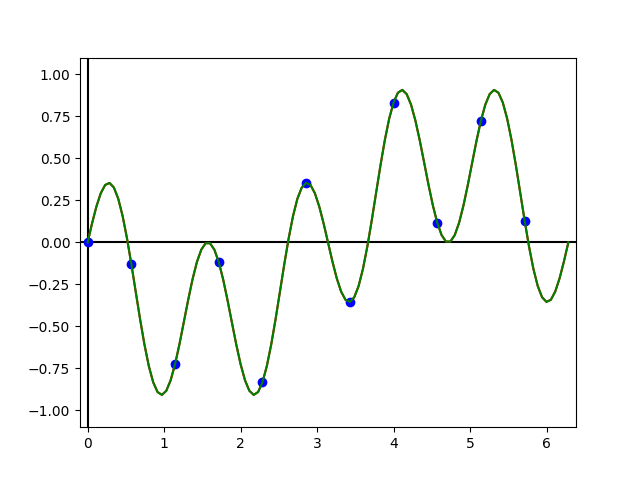
\includegraphics[width=.8\textwidth]{hw5_p6_fig1}
	\label{hw5_p6_fig1}
	\centering
\end{figure}

\begin{figure}[h]
	\caption{Error of the trigonometric interpolation of the function $f(t)=\sin(2t)\cos(3t)$}
	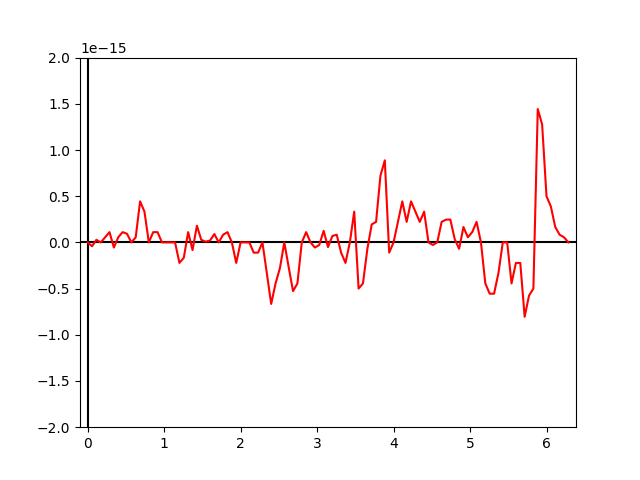
\includegraphics[width=.8\textwidth]{hw5_p6_fig2}
	\label{hw5_p6_fig2}
	\centering
\end{figure}

\problem{6 (c)} In figure (\ref{hw5_p6_fig3}) is the plot of the trigonometric interpolant of the function $f(t) = \sin(20 e^{\cos(t-\frac{1}{2})})$ through $101$ equally spaced sample points. In figure (\ref{hw5_p6_fig4}) is the error of the trigonometric interpolation. It is less than $3 \times 10^{-6}$ at all points in our interval. In figure (\ref{hw5_p6_fig5}) is the error of the piecewise cubic spline interpolated at the Chebyshev points. While the error stays below 0.01, it is not as good an approximation as the trigonometric interpolation. Since the choice of the Chebyshev points makes the best approximation for the piecewise cubic spline, we can say for certain that the trigonometric interpolation is better than any peicewise cubic spline approximation of this function.

\begin{figure}[h]
	\caption{Trigonometric interpolation of $f(t) = \sin(20 e^{\cos(t-\tfrac{1}{2})})$ at 101 equally spaced sample points}
	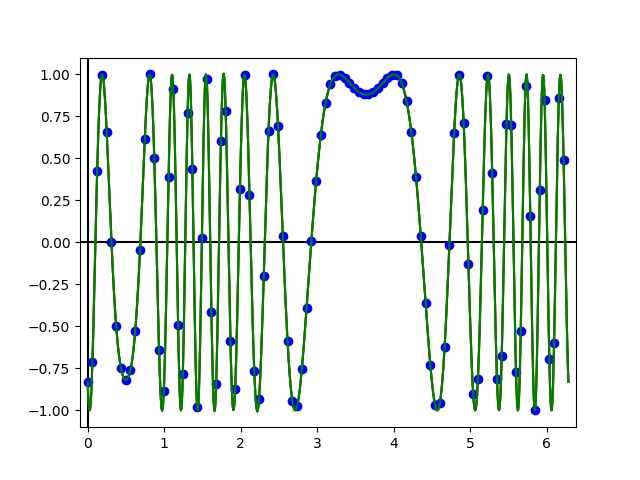
\includegraphics[width=.8\textwidth]{hw5_p6_fig3}
	\label{hw5_p6_fig3}
	\centering
\end{figure}

\begin{figure}[h]
	\caption{Error of the trigonometric interpolant of $f(t) = \sin(20 e^{\cos(t-\tfrac{1}{2})})$ at 101 equally spaced sample points}
	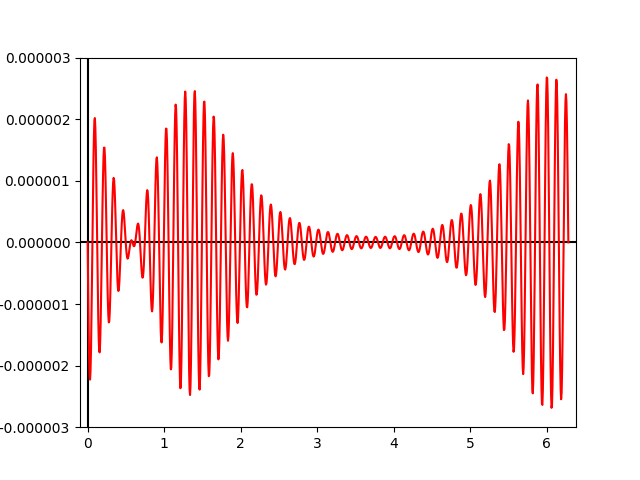
\includegraphics[width=.8\textwidth]{hw5_p6_fig4}
	\label{hw5_p6_fig4}
	\centering
\end{figure}

\begin{figure}[h]
	\caption{Error of the global interpolant of $f(t) = \sin(20 e^{\cos(t-\tfrac{1}{2})})$ at 101 Chebyshev points}
	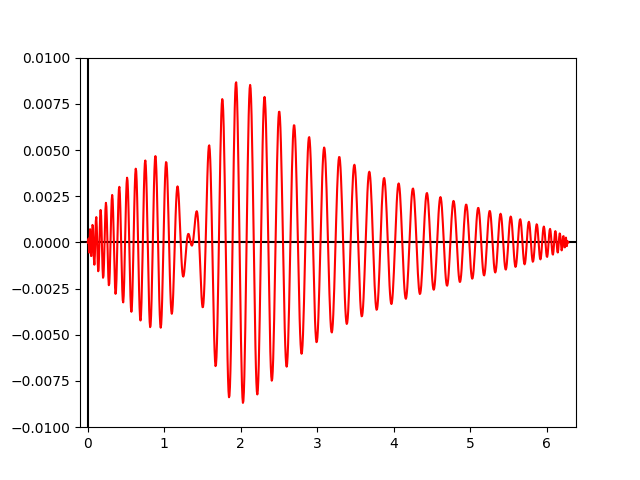
\includegraphics[width=.8\textwidth]{hw5_p6_fig5}
	\label{hw5_p6_fig5}
	\centering
\end{figure}

\problem{6 (d)} In figure (\ref{hw5_p6_fig6}) can be seen the trigonometric interpolation for the square wave of period $2\pi$ sampled at $101$ equally spaced samples over this interval and interpolated/extrapolated over the interval $[0,6\pi]$. The Gibb's Phenomenon can be seen near the clifs in the square wave. The maximum value (amplitude) of the trigonometric interpolant is approximately $1.2728$ which is close to the expected fixed constant $1.28114$. 

\begin{figure}[h]
	\caption{Square wave of period $2\pi$ and the trigonometric interpolant}
	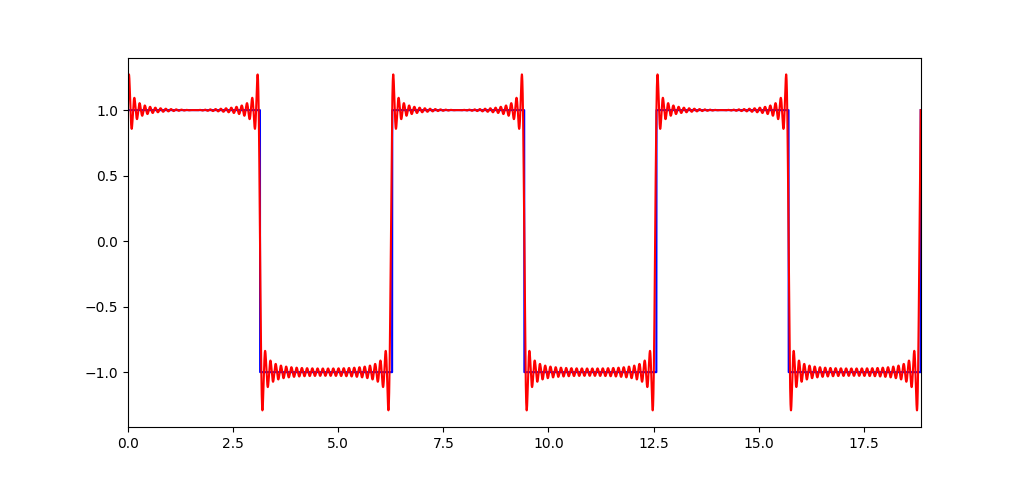
\includegraphics[width=1.0\textwidth]{hw5_p6_fig6}
	\label{hw5_p6_fig6}
	\centering
\end{figure}

\end{document}
